%!TEX program = xelatex
% ============================================================================
% ΔΙΠΛΩΜΑΤΙΚΗ ΕΡΓΑΣΙΑ - ΠΟΛΥΤΕΧΝΕΙΟ ΚΡΗΤΗΣ
% Σχεδιασμός και Υλοποίηση Πλατφόρμας Διαχείρισης Τουριστικών Καταλυμάτων
% με Έμφαση στο Rapid Development και την Ενσωμάτωση LLMs
% 
% Συγγραφέας: Θεόδωρος Μπάρκας
% Επιβλέπων: Καθ. Μιχαήλ Γ. Λαγουδάκης
% Ημερομηνία: Νοέμβριος 2025
% ============================================================================

\documentclass[12pt,a4paper,twoside,openright]{report}

% ============================================================================
% PACKAGES
% ============================================================================

% Language and Encoding
\usepackage{fontspec}
\usepackage{polyglossia}
\setdefaultlanguage{greek}
\setotherlanguage{english}

% Use system fonts - Helvetica has Greek support
\defaultfontfeatures{Ligatures=TeX}
\setmainfont{Helvetica}
\setsansfont{Helvetica Neue}
\setmonofont{Menlo}[Scale=0.85]

% Define Greek font explicitly
\newfontfamily\greekfont{Helvetica}
\newfontfamily\greekfontsf{Helvetica Neue}
\newfontfamily\greekfonttt{Menlo}[Script=Default,Scale=0.85]

% Page Layout
\usepackage[
    top=2.5cm,
    bottom=2.5cm,
    left=3cm,
    right=2.5cm,
    headheight=15pt
]{geometry}

% Headers and Footers
\usepackage{fancyhdr}
\pagestyle{fancy}
\fancyhf{}
\fancyhead[LE,RO]{\thepage}
\fancyhead[RE]{\leftmark}
\fancyhead[LO]{\rightmark}
\renewcommand{\headrulewidth}{0.4pt}

% Graphics and Figures
\usepackage{graphicx}
\usepackage{float}
\usepackage{subcaption}
\graphicspath{{./images/}{./erd/}{./presentation_assets/}}

% Tables
\usepackage{booktabs}
\usepackage{longtable}
\usepackage{array}
\usepackage{multirow}
\usepackage{tabularx}
\newcolumntype{L}[1]{>{\raggedright\arraybackslash}p{#1}}
\newcolumntype{C}[1]{>{\centering\arraybackslash}p{#1}}
\newcolumntype{R}[1]{>{\raggedleft\arraybackslash}p{#1}}

% Code Listings
\usepackage{listings}
\usepackage{xcolor}

\definecolor{codebg}{RGB}{248,248,248}
\definecolor{codeframe}{RGB}{200,200,200}
\definecolor{codekeyword}{RGB}{0,0,180}
\definecolor{codecomment}{RGB}{0,128,0}
\definecolor{codestring}{RGB}{163,21,21}

\lstdefinestyle{typescript}{
    language=Java,
    basicstyle=\footnotesize\ttfamily,
    backgroundcolor=\color{codebg},
    frame=single,
    rulecolor=\color{codeframe},
    keywordstyle=\color{codekeyword}\bfseries,
    commentstyle=\color{codecomment}\itshape,
    stringstyle=\color{codestring},
    showstringspaces=false,
    breaklines=true,
    breakatwhitespace=true,
    tabsize=2,
    numbers=left,
    numberstyle=\tiny\color{gray},
    numbersep=8pt,
    xleftmargin=15pt,
    framexleftmargin=15pt,
    morekeywords={async,await,const,let,export,import,from,type,interface,extends,implements,return,if,else,for,while,try,catch,throw,new,function,class,static,private,public,protected,readonly},
    literate={=>}{{$\Rightarrow$}}1
}

\lstdefinestyle{text}{
    basicstyle=\footnotesize\ttfamily,
    backgroundcolor=\color{codebg},
    frame=single,
    rulecolor=\color{codeframe},
    breaklines=true,
    breakatwhitespace=true,
    tabsize=2,
    xleftmargin=15pt,
    framexleftmargin=15pt,
}

\lstset{style=typescript}

% Mathematics
\usepackage{amsmath}
\usepackage{amssymb}

% Hyperlinks and References
\usepackage{hyperref}
\hypersetup{
    colorlinks=true,
    linkcolor=blue!60!black,
    citecolor=green!50!black,
    urlcolor=blue!70!black,
    pdftitle={Σχεδιασμός και Υλοποίηση Πλατφόρμας Διαχείρισης Τουριστικών Καταλυμάτων},
    pdfauthor={Θεόδωρος Μπάρκας},
}

% Bibliography
\usepackage[backend=biber,style=numeric,sorting=none]{biblatex}
\addbibresource{references.bib}

% Captions
\usepackage{caption}
\captionsetup{
    font=small,
    labelfont=bf,
    format=hang,
    margin=10pt
}

% Spacing
\usepackage{setspace}
\onehalfspacing

% Chapter and Section Formatting
\usepackage{titlesec}
\titleformat{\chapter}[display]
    {\normalfont\huge\bfseries}
    {\chaptertitlename\ \thechapter}
    {20pt}
    {\Huge}
\titlespacing*{\chapter}{0pt}{-20pt}{40pt}

% Table of Contents Depth
\setcounter{tocdepth}{3}
\setcounter{secnumdepth}{3}

% Custom Commands
\newcommand{\code}[1]{\texttt{#1}}
\newcommand{\emphasis}[1]{\textit{#1}}
\newcommand{\important}[1]{\textbf{#1}}

% ============================================================================
% DOCUMENT
% ============================================================================

\begin{document}

% ============================================================================
% TITLE PAGE
% ============================================================================
\begin{titlepage}
    \centering
    \vspace*{1cm}
    
    {\large\bfseries ΠΟΛΥΤΕΧΝΕΙΟ ΚΡΗΤΗΣ}\\[0.3cm]
    {\large ΣΧΟΛΗ ΗΛΕΚΤΡΟΛΟΓΩΝ ΜΗΧΑΝΙΚΩΝ ΚΑΙ ΜΗΧΑΝΙΚΩΝ ΥΠΟΛΟΓΙΣΤΩΝ}\\[2cm]
    
    \rule{\textwidth}{1.5pt}\\[0.5cm]
    {\LARGE\bfseries ΣΧΕΔΙΑΣΜΟΣ ΚΑΙ ΥΛΟΠΟΙΗΣΗ ΠΛΑΤΦΟΡΜΑΣ ΔΙΑΧΕΙΡΙΣΗΣ ΤΟΥΡΙΣΤΙΚΩΝ ΚΑΤΑΛΥΜΑΤΩΝ ΜΕ ΕΜΦΑΣΗ ΣΤΟ RAPID DEVELOPMENT ΚΑΙ ΤΗΝ ΕΝΣΩΜΑΤΩΣΗ LLMs}\\[0.5cm]
    \rule{\textwidth}{1.5pt}\\[2cm]
    
    {\Large ΔΙΠΛΩΜΑΤΙΚΗ ΕΡΓΑΣΙΑ}\\[2cm]
    
    {\Large\bfseries ΘΕΟΔΩΡΟΣ ΜΠΑΡΚΑΣ}\\[3cm]
    
    \vfill
    
    {\large ΧΑΝΙΑ, ΝΟΕΜΒΡΙΟΣ 2025}
\end{titlepage}

% ============================================================================
% COPYRIGHT PAGE
% ============================================================================
\thispagestyle{empty}
\vspace*{\fill}

\noindent\textbf{ΠΝΕΥΜΑΤΙΚΑ ΔΙΚΑΙΩΜΑΤΑ}

\vspace{0.5cm}

\noindent«Απαγορεύεται η αντιγραφή, αποθήκευση και διανομή της παρούσας εργασίας, εξ ολοκλήρου ή τμήματος αυτής, για εμπορικό σκοπό. Επιτρέπεται η ανατύπωση, αποθήκευση και διανομή για μη κερδοσκοπικό σκοπό, εκπαιδευτικού ή ερευνητικού χαρακτήρα, με την προϋπόθεση να αναφέρεται η πηγή προέλευσης. Ερωτήματα που αφορούν τη χρήση της εργασίας για άλλη χρήση θα πρέπει να απευθύνονται προς τον συγγραφέα.

\vspace{0.3cm}

\noindent Οι απόψεις και τα συμπεράσματα που περιέχονται σε αυτό το έγγραφο εκφράζουν τον συγγραφέα και δεν πρέπει να ερμηνευθεί ότι αντιπροσωπεύουν τις επίσημες θέσεις του Πολυτεχνείου Κρήτης.»

\vspace*{\fill}
\clearpage

% ============================================================================
% COMMITTEE PAGE
% ============================================================================
\thispagestyle{empty}
\vspace*{3cm}

\begin{center}
    {\Large\bfseries ΕΞΕΤΑΣΤΙΚΗ ΕΠΙΤΡΟΠΗ}
\end{center}

\vspace{2cm}

\begin{enumerate}
    \item \textbf{Καθηγητής Μιχαήλ Γ. Λαγουδάκης} (Επιβλέπων)\\
    Πολυτεχνείο Κρήτης, Σχολή Ηλεκτρολόγων Μηχανικών και Μηχανικών Υπολογιστών
    
    \vspace{1cm}
    
    \item \textbf{Καθηγητής Αντώνιος Δεληγιαννάκης}\\
    Πολυτεχνείο Κρήτης, Σχολή Ηλεκτρολόγων Μηχανικών και Μηχανικών Υπολογιστών
    
    \vspace{1cm}
    
    \item \textbf{Αναπληρωτής Καθηγητής Βασίλειος Σαμολαδάς}\\
    Πολυτεχνείο Κρήτης, Σχολή Ηλεκτρολόγων Μηχανικών και Μηχανικών Υπολογιστών
\end{enumerate}

\vspace*{\fill}
\clearpage

% ============================================================================
% ABSTRACT (GREEK)
% ============================================================================
\chapter*{Περίληψη}
\addcontentsline{toc}{chapter}{Περίληψη}

Η παρούσα διπλωματική εργασία πραγματεύεται τον σχεδιασμό και την υλοποίηση της πλατφόρμας «Lunarety V2», ενός προηγμένου συστήματος διαχείρισης τουριστικών καταλυμάτων (Property Management System -- PMS) που αξιοποιεί σύγχρονες τεχνολογίες για να προσφέρει λύσεις Rapid Development και ενσωμάτωση Τεχνητής Νοημοσύνης (LLMs). Σκοπός της εργασίας είναι η κάλυψη του κενού που υπάρχει στην αγορά για ένα εργαλείο που απευθύνεται σε διαχειριστές ακινήτων (Managers) οι οποίοι επιβλέπουν πολλαπλούς ιδιοκτήτες (Owners), προσφέροντας διαφάνεια, αυτοματισμό και ευκολία χρήσης που λείπει από τα παραδοσιακά Channel Managers.

Η μεθοδολογία ανάπτυξης βασίστηκε στη χρήση του PayloadCMS v3.0, το οποίο λειτουργεί ως ένα πλήρες backend framework εντός του Next.js, προσφέροντας Code-First ορισμό δομών δεδομένων και ισχυρή τυποποίηση μέσω TypeScript. Η βάση δεδομένων υλοποιήθηκε σε PostgreSQL με χρήση Drizzle ORM, εξασφαλίζοντας ακεραιότητα και ταχύτητα. Η πλατφόρμα ακολουθεί αρχιτεκτονική Monorepo και είναι σχεδιασμένη για Serverless Deployment (π.χ. Vercel), επιτρέποντας στους διαχειριστές να ξεκινούν με μηδενικό κόστος υποδομής και να κλιμακώνονται ανάλογα με τις ανάγκες τους.

Κεντρικό στοιχείο της καινοτομίας αποτελεί η ενσωμάτωση Large Language Models (LLMs) μέσω του Vercel AI SDK και του OpenRouter, προσφέροντας έξυπνες λειτουργίες σε πολλαπλά επίπεδα. Επιπλέον, αναπτύχθηκε ένας μηχανισμός «Auto Actions» για την πλήρη αυτοματοποίηση της επικοινωνίας μέσω πολλαπλών καναλιών (Email, OTA Messages, Telegram).

Η εργασία συνεισφέρει στην κατανόηση του τρόπου με τον οποίο οι σύγχρονες αρχιτεκτονικές λογισμικού και τα εργαλεία Rapid Development μπορούν να μετασχηματίσουν επιχειρησιακές διαδικασίες, προσφέροντας λύσεις υψηλής αξίας με μειωμένο χρόνο ανάπτυξης και συντήρησης.

\vspace{1cm}
\noindent\textbf{Λέξεις-κλειδιά:} Property Management System, Rapid Development, Large Language Models, PayloadCMS, Next.js, TypeScript, Serverless, Channel Manager, Auto Actions

\clearpage

% ============================================================================
% ABSTRACT (ENGLISH)
% ============================================================================
\chapter*{Abstract}
\addcontentsline{toc}{chapter}{Abstract}

\begin{english}
This diploma thesis deals with the design and implementation of the «Lunarety V2» platform, an advanced Property Management System (PMS) that leverages modern technologies to offer Rapid Development solutions and Large Language Model (LLM) integration. The purpose of this work is to bridge the market gap for a tool tailored to Property Managers overseeing multiple Owners, offering transparency, automation, and ease of use often missing from traditional Channel Managers.

The development methodology was based on PayloadCMS v3.0, acting as a full backend framework within Next.js, offering Code-First data structure definitions and strong typing via TypeScript. The database was implemented in PostgreSQL using Drizzle ORM, ensuring data integrity and performance. The platform follows a Monorepo architecture and is designed for Serverless Deployment (e.g., Vercel), allowing managers to start with zero infrastructure costs and scale as needed.

A key innovation element is the integration of Large Language Models (LLMs) via Vercel AI SDK and OpenRouter, offering smart features at multiple levels. Furthermore, an «Auto Actions» mechanism was developed to fully automate communication through multiple channels (Email, OTA Messages, Telegram).

This work contributes to understanding how modern software architectures and Rapid Development tools can transform business processes, delivering high-value solutions with reduced development and maintenance time.

\vspace{1cm}
\noindent\textbf{Keywords:} Property Management System, Rapid Development, Large Language Models, PayloadCMS, Next.js, TypeScript, Serverless, Channel Manager, Auto Actions
\end{english}

\clearpage

% ============================================================================
% PREFACE / ACKNOWLEDGEMENTS
% ============================================================================
\chapter*{Πρόλογος}
\addcontentsline{toc}{chapter}{Πρόλογος}

Θα ήθελα να ευχαριστήσω... (Placeholder for Acknowledgements)

\clearpage

% ============================================================================
% TABLE OF CONTENTS
% ============================================================================
\tableofcontents
\clearpage

\listoffigures
\addcontentsline{toc}{chapter}{Κατάλογος Εικόνων}
\clearpage

\listoftables
\addcontentsline{toc}{chapter}{Κατάλογος Πινάκων}
\clearpage

% ============================================================================
% CHAPTER 1: INTRODUCTION
% ============================================================================
\chapter{Εισαγωγή}
\label{chap:introduction}

\section{Αντικείμενο της Μελέτης}
\label{sec:subject}

Το αντικείμενο της παρούσας διπλωματικής εργασίας είναι ο σχεδιασμός και η ανάπτυξη ενός ολοκληρωμένου πληροφοριακού συστήματος, του «Lunarety V2», για τη διαχείριση τουριστικών καταλυμάτων. Η πλατφόρμα δεν αποτελεί απλώς ένα ακόμη PMS, αλλά μια ολιστική λύση που στοχεύει στην κεντρικοποίηση των λειτουργιών που απαιτούνται από επαγγελματίες διαχειριστές (Managers) και τους πελάτες τους, τους ιδιοκτήτες ακινήτων (Owners). Πέρα από τις βασικές λειτουργίες διαχείρισης κρατήσεων και συγχρονισμού ημερολογίων, η πλατφόρμα ενσωματώνει προηγμένες δυνατότητες Τεχνητής Νοημοσύνης (LLMs) για την υποβοήθηση της επικοινωνίας και την παροχή έξυπνων υπηρεσιών.

\section{Σκοπός της Διπλωματικής Εργασίας}
\label{sec:purpose}

Ο κύριος σκοπός της εργασίας είναι η δημιουργία ενός εργαλείου που μειώνει δραστικά τον διοικητικό φόρτο και εκσυγχρονίζει τις διαδικασίες διαχείρισης. Ειδικότερα, επιδιώκεται:

\begin{itemize}
    \item Η δημιουργία ενός robust συστήματος διαχείρισης σχέσεων Manager-Owner, προσφέροντας διαφάνεια και αυτοματοποιημένη ενημέρωση.
    \item Η ενσωμάτωση δυνατοτήτων LLM (Large Language Models) τόσο για την υποβοήθηση των χρηστών στη σύνταξη μηνυμάτων όσο και για την παροχή smart features στους επισκέπτες μέσω των ιστοσελίδων των καταλυμάτων.
    \item Η υλοποίηση ενός ευέλικτου συστήματος «Auto Actions» τριών επιπέδων για την πλήρη αυτοματοποίηση των εργασιών.
    \item Η απρόσκοπτη διασύνδεση με τον Channel Manager «Beds24», με αρχιτεκτονική πρόβλεψη για μελλοντική προσθήκη άλλων παρόχων.
\end{itemize}

\section{Το Κενό στην Αγορά: Managers και Owners}
\label{sec:market-gap}

Η παρούσα εργασία απευθύνεται κυρίως σε επαγγελματίες Property Managers που διαχειρίζονται χαρτοφυλάκια ακινήτων που ανήκουν σε τρίτους (Owners). Στην τρέχουσα αγορά, παρατηρείται ένα σημαντικό κενό:

\begin{itemize}
    \item Οι Managers συχνά αναγκάζονται να χρησιμοποιούν πολύπλοκα λογισμικά Channel Managers, τα οποία είναι δύσχρηστα για τους Owners ή το απλό προσωπικό.
    \item Η ενημέρωση των Owners για κρατήσεις, πληρότητες και οικονομικά στοιχεία γίνεται συχνά χειροκίνητα (τηλέφωνα, excel, emails), οδηγώντας σε λάθη και καθυστερήσεις.
    \item Η δημιουργία λογαριασμών για Owners μέσα στα υπάρχοντα Channel Managers είναι συχνά δαπανηρή ή πολύπλοκη διαδικασία.
\end{itemize}

Το Lunarety V2 έρχεται να καλύψει αυτό το κενό, προσφέροντας μια ενδιάμεση, φιλική προς τον χρήστη πλατφόρμα, όπου ο Manager ορίζει τα δικαιώματα, τις συνδρομές και την πρόσβαση των Owners, παρέχοντάς τους ακριβώς την πληροφορία που χρειάζονται σε πραγματικό χρόνο.

\section{Συνεισφορά στο Rapid Development}
\label{sec:rapid-dev-contribution}

Πέρα από την επιχειρησιακή της αξία, η εργασία αυτή αποτελεί μελέτη περίπτωσης για το πώς σύγχρονες τεχνολογίες (Next.js, PayloadCMS, Serverless) συμβάλλουν στο Rapid Application Development (RAD)~\cite{rapid_development}. Η δυνατότητα γρήγορης ανάπτυξης, εύκολου deployment (Serverless)~\cite{vercel} και άμεσης προσαρμογής (Code-First schema) επιτρέπει σε μικρές ομάδες ή μεμονωμένους developers να παράγουν λογισμικό επιχειρησιακού επιπέδου (Enterprise Grade) σε ελάχιστο χρόνο.

% ============================================================================
% CHAPTER 2: THEORETICAL BACKGROUND
% ============================================================================
\chapter{Θεωρητικό Υπόβαθρο}
\label{chap:theory}

\section{Σύγχρονες Αρχιτεκτονικές Web}
\label{sec:modern-architectures}

\begin{figure}[H]
    \centering
    \includegraphics[width=0.9\textwidth]{tech_stack_logos.png}
    \caption{Το τεχνολογικό stack της πλατφόρμας (Next.js, PayloadCMS, PostgreSQL, κ.α.).}
    \label{fig:tech-stack}
\end{figure}

\subsection{TypeScript και Type Consistency}
\label{subsec:typescript}

Η επιλογή της TypeScript έναντι της JavaScript αποτέλεσε μονόδρομο για την ανάπτυξη μιας σύγχρονης, κλιμακώσιμης εφαρμογής~\cite{typescript}. Η στατική τυποποίηση (static typing) που προσφέρει εξασφαλίζει «Type Consistency» σε όλο το εύρος της εφαρμογής (Fullstack). Αυτό σημαίνει ότι τα δεδομένα που επιστρέφει το Backend είναι εγγυημένα συμβατά με αυτά που περιμένει το Frontend, μειώνοντας δραματικά τα runtime errors και επιταχύνοντας την ανάπτυξη μέσω του IntelliSense.

\subsection{PayloadCMS: Backend Framework vs CMS}
\label{subsec:payloadcms}

Το PayloadCMS (ειδικά από την έκδοση 3.0 και μετά) διαφοροποιείται σημαντικά από τα παραδοσιακά CMS (όπως το WordPress ή το Strapi)~\cite{payloadcms}. Λειτουργεί πρωτίστως ως ένα Backend Framework που τρέχει εντός του Next.js, παρόμοια με το Django ή το Laravel, αλλά με τη δύναμη του TypeScript.

\begin{description}
    \item[Code-First Collections:] Οι δομές δεδομένων (Collections) ορίζονται αποκλειστικά μέσω κώδικα (TypeScript objects), λειτουργώντας ταυτόχρονα ως σχήμα βάσης δεδομένων, μοντέλο API και διεπαφή διαχείρισης.
    \item[Next.js Integration:] Το backend (Admin panel, API routes, Auth) είναι ενσωματωμένο στην εφαρμογή Next.js, μετατρέποντάς την σε μια full-stack λύση χωρίς την ανάγκη ξεχωριστού server.
\end{description}

\subsection{Next.js, Server Actions και Monorepo}
\label{subsec:nextjs}

Το Next.js επιλέχθηκε όχι μόνο για τις δυνατότητες Rendering (SSR, SSG) αλλά και για την άριστη συμβατότητά του με Serverless υποδομές~\cite{nextjs,serverless}.

\begin{description}
    \item[Server Actions:] Μια κρίσιμη λειτουργία που επιτρέπει στο Frontend να καλεί συναρτήσεις του Backend απευθείας, χωρίς την ανάγκη ρητού ορισμού API Endpoints. Αυτό απλοποιεί τη διαχείριση δεδομένων και διατηρεί την τυποποίηση (types) από άκρη σε άκρη.
    \item[Monorepo:] Η διατήρηση όλου του κώδικα (Frontend, Backend, Webhooks) σε ένα ενιαίο Repository επιτρέπει την κοινή χρήση τύπων και utilities, εξαλείφοντας την ανάγκη για συγχρονισμό μεταξύ διαφορετικών projects.
\end{description}

\subsection{PostgreSQL και Drizzle ORM}
\label{subsec:postgresql}

Η πλατφόρμα βασίζεται στην PostgreSQL~\cite{postgresql}, μια ισχυρή σχεσιακή βάση δεδομένων. Η επικοινωνία με τη βάση γίνεται μέσω του Drizzle ORM~\cite{drizzle}, το οποίο είναι πλήρως συμβατό με το PayloadCMS.

\begin{description}
    \item[Low-Level Capabilities:] Το Drizzle επιτρέπει στον developer να γράψει σύνθετα SQL queries όταν οι abstraction layers του CMS δεν επαρκούν, προσφέροντας απόλυτο έλεγχο στην απόδοση.
    \item[Type Safety:] Πλήρης τυποποίηση των queries βάσει του σχήματος της βάσης.
\end{description}

\subsection{Shadcn UI, React και Zustand}
\label{subsec:shadcn}

Για το User Interface χρησιμοποιήθηκε το Shadcn UI~\cite{shadcn}, το οποίο διαφέρει από τις παραδοσιακές βιβλιοθήκες (όπως το Material UI) καθώς δεν είναι ένα npm package, αλλά κώδικας που αντιγράφεται μέσα στο project. Αυτό δίνει απόλυτη ελευθερία παραμετροποίησης.

\begin{description}
    \item[React:] Η βάση του frontend για τη δημιουργία επαναχρησιμοποιήσιμων components~\cite{react}.
    \item[Zustand:] Χρησιμοποιήθηκε για τη διαχείριση της κατάστασης (state management) της εφαρμογής~\cite{zustand}, προσφέροντας μια πιο απλή και ελαφριά εναλλακτική στο Redux.
\end{description}

\subsection{Swagger/OpenAPI και Code Generation}
\label{subsec:openapi}

Για την επικοινωνία μεταξύ της Πλατφόρμας και των Websites, χρησιμοποιήθηκε το πρότυπο OpenAPI (Swagger)~\cite{openapi}.

\begin{description}
    \item[Generation:] Η βιβλιοθήκη \code{next-swagger-doc} παράγει αυτόματα το documentation του API.
    \item[Client:] Η βιβλιοθήκη \code{openapi-typescript-codegen} χρησιμοποιείται στο Website project για να παράγει έναν πλήρως τυποποιημένο client (SDK), εξασφαλίζοντας ότι το Website είναι πάντα συγχρονισμένο με τις αλλαγές στο API της πλατφόρμας.
\end{description}

\section{Large Language Models (LLMs)}
\label{sec:llms}

Η ενσωμάτωση LLMs (μέσω API όπως OpenAI ή Anthropic) μεταμορφώνει τις εφαρμογές από στατικά εργαλεία σε έξυπνους βοηθούς~\cite{llm_applications}. Στο πλαίσιο του PMS, τα LLMs μπορούν να αναλύσουν το context μιας κράτησης και να προτείνουν απαντήσεις, να μεταφράσουν μηνύματα ή να λειτουργήσουν ως virtual concierges στις ιστοσελίδες των καταλυμάτων.

\subsection{Vercel AI SDK και Streaming}
\label{subsec:vercel-ai}

Για την υλοποίηση των AI λειτουργιών χρησιμοποιήθηκε το \textbf{Vercel AI SDK (v5)}~\cite{vercelai}. Το SDK αυτό επιλέχθηκε διότι απλοποιεί δραματικά τη διαδικασία του \textbf{Streaming} (ροή δεδομένων), επιτρέποντας στο UI να εμφανίζει την απάντηση του AI σταδιακά (λέξη-λέξη) καθώς παράγεται, βελτιώνοντας την εμπειρία χρήστη.

\subsection{OpenRouter και Πρόσβαση σε Μοντέλα}
\label{subsec:openrouter}

Η πλατφόρμα δεν συνδέεται απευθείας με έναν πάροχο (π.χ. OpenAI), αλλά χρησιμοποιεί το \textbf{OpenRouter}~\cite{openrouter}. Το OpenRouter λειτουργεί ως ένας ενδιάμεσος κόμβος (gateway) που παρέχει πρόσβαση σε πληθώρα μοντέλων (GPT-4, Claude 3.5 Sonnet, Llama 3, κ.α.) μέσω ενός ενιαίου API. Αυτό δίνει την ευελιξία στον χρήστη να επιλέξει το μοντέλο που ταιριάζει καλύτερα στις ανάγκες και το budget του, χωρίς αλλαγές στον κώδικα.

\section{Channel Managers και Διασυνδεσιμότητα}
\label{sec:channel-managers}

Η επιλογή του \textbf{Beds24}~\cite{beds24api} ως Channel Manager δεν ήταν τυχαία. Επιλέχθηκε διότι:

\begin{enumerate}
    \item \textbf{Δημοφιλία \& Κόστος:} Είναι μια από τις πιο διαδεδομένες και οικονομικές λύσεις στην αγορά~\cite{pms_systems}.
    \item \textbf{Modern API:} Διαθέτει ένα σύγχρονο, comprehensive API με υποστήριξη OpenAPI, το οποίο επιτρέπει την εύκολη παραγωγή κώδικα (μέσω \code{swagger-typescript-api}) και την άμεση προσαρμογή σε μελλοντικά updates.
\end{enumerate}

% ============================================================================
% CHAPTER 3: METHODOLOGY & REQUIREMENTS ANALYSIS
% ============================================================================
\chapter{Μεθοδολογία και Ανάλυση Απαιτήσεων}
\label{chap:methodology}

\section{Ρόλοι και Ιεραρχία Χρηστών}
\label{sec:user-hierarchy}

Το σύστημα σχεδιάστηκε με γνώμονα την ιεραρχία Manager-Owner, υλοποιώντας ένα εύκαμπτο μοντέλο δικαιωμάτων που επιτρέπει τον έλεγχο σε κάθε επίπεδο.

\subsection{Τύποι Χρηστών (User Types)}
\label{subsec:user-types}

Η πλατφόρμα υποστηρίζει τέσσερις διακριτούς τύπους χρηστών, όπως παρουσιάζονται στον Πίνακα~\ref{tab:user-types}.

\begin{table}[H]
\centering
\caption{Τύποι χρηστών της πλατφόρμας}
\label{tab:user-types}
\begin{tabular}{@{}llll@{}}
\toprule
\textbf{User Type} & \textbf{Περιγραφή} & \textbf{Parent} & \textbf{Children} \\
\midrule
\code{platform-user} & Administrators πλατφόρμας & Κανένας & Managers \\
\code{manager} & Property Managers & Platform & Owners, Staff \\
\code{owner} & Ιδιοκτήτες ακινήτων & Manager & Staff \\
\code{stuff} & Προσωπικό & Owner/Manager & Κανένας \\
\bottomrule
\end{tabular}
\end{table}

\paragraph{Platform Users (Admins):}
\begin{itemize}
    \item Πλήρης πρόσβαση σε όλα τα δεδομένα της πλατφόρμας (Admin View)
    \item Δημιουργία και διαχείριση Plans (πλάνα χρέωσης)
    \item Εποπτεία όλων των Managers, χωρίς να είναι «γονείς» τους ιεραρχικά, αλλά έχοντας δυνατότητα διαχείρισης.
\end{itemize}

\paragraph{Managers:}
\begin{itemize}
    \item Σύνδεση με Channel Manager (Beds24)
    \item Εισαγωγή και διαχείριση Properties
    \item Δημιουργία Owners και Staff
    \item Ορισμός δικαιωμάτων για τους υφισταμένους
    \item Δυνατότητα παραμετροποίησης των δικών τους access configurations
    \item Δημιουργία και διαχείριση Auto Actions
    \item Δημιουργία Websites για τα ακίνητα
\end{itemize}

\paragraph{Owners:}
\begin{itemize}
    \item Προβολή/επεξεργασία μόνο των ακινήτων που τους έχουν ανατεθεί
    \item Δικαιώματα καθορίζονται πλήρως από τον Manager
    \item Δημιουργία Staff που ανήκουν σε αυτούς
\end{itemize}

\paragraph{Staff:}
\begin{itemize}
    \item Ελάχιστα δικαιώματα (συνήθως view-only)
    \item Δεν μπορούν να δημιουργήσουν άλλους χρήστες
    \item Χρήσιμοι για εργασίες καθαρισμού, check-in, κ.λπ.
\end{itemize}

\subsection{Ιεραρχικές Σχέσεις και Billing}
\label{subsec:hierarchical-relations}

Κάθε Owner ανήκει σε έναν Manager/Platform-User, ενώ το Staff μπορεί να ανήκει σε Manager ή Owner. Η σχέση αυτή καθορίζει την πρόσβαση και τη ροή των χρεώσεων. Κάθε Manager και Owner συνδέεται με ένα Plan που καθορίζει τις χρεώσεις και τα features.

\begin{figure}[H]
    \centering
    \includegraphics[width=0.8\textwidth]{user_hierarchy.png}
    \caption{Ιεραρχική δομή ρόλων χρηστών στην πλατφόρμα.}
    \label{fig:user-hierarchy}
\end{figure}

\section{Αρχιτεκτονική Συστήματος (Monorepo)}
\label{sec:system-architecture}

Η πλατφόρμα υλοποιείται ως Monorepo, το οποίο εξασφαλίζει συνοχή μεταξύ των διαφορετικών components και διευκολύνει την κοινή χρήση τύπων και utilities.

\subsection{Δομή Monorepo}
\label{subsec:monorepo-structure}

\begin{lstlisting}[style=text,caption={Δομή καταλόγων του Monorepo}]
lunarety-v2/
├── src/
│   ├── app/                    # Next.js App Router
│   │   ├── (frontend)/         # Frontend routes
│   │   └── (payload)/          # PayloadCMS admin routes
│   ├── apis/                   # External API integrations
│   │   └── channel-managers/   # Beds24 API, DTOs, sync
│   ├── collections/            # PayloadCMS collections
│   ├── crons/                  # Scheduled jobs
│   ├── endpoints/              # Custom API endpoints
│   ├── lib/                    # Shared utilities
│   └── payload.config.ts       # PayloadCMS configuration
├── lunarety-v2-website/        # Website template
└── package.json
\end{lstlisting}

\subsection{Βασικά Components}
\label{subsec:basic-components}

\paragraph{PayloadCMS Core:}
\begin{itemize}
    \item Headless CMS με PostgreSQL backend
    \item Αυτόματη δημιουργία REST και GraphQL API
    \item Admin panel για διαχείριση δεδομένων
    \item Type-safe collection definitions
\end{itemize}

\paragraph{Next.js App Router:}
\begin{itemize}
    \item Server-side rendering για SEO
    \item Server Actions για data mutations
    \item Middleware για authentication
    \item Dynamic routing για Calendar, Messages, Settings
\end{itemize}

\paragraph{Channel Manager API Layer:}
\begin{itemize}
    \item \code{ChannelManagerApi} object -- central export point
    \item DTOs για μετατροπή Beds24 $\leftrightarrow$ Payload formats
    \item Abstraction layer για μελλοντική υποστήριξη άλλων Channel Managers
\end{itemize}

Το κρίσιμο σημείο αυτής της αρχιτεκτονικής είναι ότι ολόκληρη η πλατφόρμα χρησιμοποιεί αυτές τις συναρτήσεις \textbf{χωρίς να είναι εξαρτημένη από το Beds24}. Οι υπόλοιπες μονάδες της εφαρμογής (hooks, cron jobs, webhooks) καλούν τα generic methods του \code{ChannelManagerApi} object, τα οποία εσωτερικά μεταφράζονται στις αντίστοιχες κλήσεις του συγκεκριμένου Channel Manager. Αυτός ο σχεδιασμός ακολουθεί το πρότυπο \textbf{Adapter Pattern}~\cite{design_patterns,software_architecture}.

\subsection{External Integrations}
\label{subsec:external-integrations}

\begin{table}[H]
\centering
\caption{External Services και Integrations}
\label{tab:integrations}
\begin{tabular}{@{}lll@{}}
\toprule
\textbf{Service} & \textbf{Σκοπός} & \textbf{Module} \\
\midrule
Beds24 API & Channel Manager & \code{apis/channel-managers/beds24/} \\
Vercel AI SDK & AI text improvements & \code{lib/ai/} \\
OpenRouter & LLM API proxy & \code{lib/ai/} \\
Telegram Bot API & User notifications & \code{lib/telegram/} \\
Resend & Email sending & \code{lib/email/} \\
\bottomrule
\end{tabular}
\end{table}

\begin{figure}[H]
    \centering
    \includegraphics[width=\textwidth]{system_architecture.png}
    \caption{Διάγραμμα αρχιτεκτονικής συστήματος (Monorepo).}
    \label{fig:system-architecture}
\end{figure}

Παράλληλα, το \code{lunarety-v2-website} αποτελεί ένα ξεχωριστό public project στο GitHub, σχεδιασμένο να λειτουργεί ως template για τις ιστοσελίδες των καταλυμάτων. Επικοινωνεί με την πλατφόρμα μέσω ενός secure API endpoint χρησιμοποιώντας \code{WEBSITE\_API\_KEY}.

\section{Μοντέλο Δεδομένων και Σχέσεις}
\label{sec:data-model}

\subsection{Κύριες Οντότητες (Collections)}
\label{subsec:collections}

Η βάση δεδομένων (PostgreSQL) οργανώνεται γύρω από τις κύριες collections που παρουσιάζονται στον Πίνακα~\ref{tab:collections}.

\begin{table}[H]
\centering
\caption{Κύριες Collections της βάσης δεδομένων}
\label{tab:collections}
\begin{tabular}{@{}L{2.5cm}L{3.5cm}L{6cm}@{}}
\toprule
\textbf{Collection} & \textbf{Περιγραφή} & \textbf{Σημαντικά Fields} \\
\midrule
\code{users} & Χρήστες πλατφόρμας & \code{type}, \code{managedBy}, \code{ownedBy}, \code{settings} \\
\code{property} & Καταλύματα & \code{manager}, \code{owner}, \code{channelPropertyId}, \code{rooms} \\
\code{bookings} & Κρατήσεις & \code{property}, \code{resource}, \code{pricing}, \code{messages} \\
\code{property-rates} & Τιμές ανά ημέρα & \code{property}, \code{date}, \code{channelRoomId}, \code{availability} \\
\code{billing} & Χρεώσεις/Τιμολόγια & \code{type}, \code{ownerDebtor}, \code{managerCreditor} \\
\code{auto-actions} & Κανόνες αυτοματισμού & \code{type}, \code{triggerType}, \code{template} \\
\code{plans} & Πλάνα χρέωσης & \code{planCommission}, \code{features} \\
\code{website} & Generated websites & \code{apiKey}, \code{type}, \code{properties} \\
\bottomrule
\end{tabular}
\end{table}

\subsection{Σχέσεις Μεταξύ Οντοτήτων}
\label{subsec:entity-relations}

\paragraph{Property $\leftrightarrow$ Users:}
\begin{itemize}
    \item Κάθε Property έχει έναν \code{manager} (υποχρεωτικό)
    \item Κάθε Property μπορεί να έχει έναν \code{owner} (προαιρετικό)
\end{itemize}

\paragraph{Bookings $\leftrightarrow$ Property $\leftrightarrow$ Users:}
\begin{itemize}
    \item Κάθε Booking ανήκει σε ένα Property
    \item Το Access control βασίζεται στη σχέση Property $\rightarrow$ Manager/Owner
\end{itemize}

\paragraph{Property Rates $\leftrightarrow$ Property $\leftrightarrow$ Bookings:}
\begin{itemize}
    \item Κάθε Rate συνδέεται με μια ημέρα και ένα δωμάτιο
    \item Τα Bookings συνδέονται με τα rates μέσω \code{relatedRates}
    \item Join field \code{bookingsStayingOnThisNight} για reverse lookup
\end{itemize}

\paragraph{Auto Actions $\leftrightarrow$ Booking $\leftrightarrow$ Users/Properties:}
\begin{itemize}
    \item Κάθε Auto Action ενεργοποιείται (Trigger) από γεγονότα που αφορούν ένα \textbf{Booking}
    \item Συνδέει και χρησιμοποιεί δεδομένα από πολλά Properties και Users
    \item Τα Properties μπορούν να «εγγραφούν» (subscribe) σε Auto Actions
\end{itemize}

\subsection{Hook System και Lifecycle}
\label{subsec:hook-system}

Το PayloadCMS παρέχει ένα ισχυρό σύστημα hooks που χρησιμοποιείται εκτενώς (Πίνακας~\ref{tab:hooks}).

\begin{table}[H]
\centering
\caption{Hook Types και χρήση στην πλατφόρμα}
\label{tab:hooks}
\begin{tabular}{@{}lll@{}}
\toprule
\textbf{Hook Type} & \textbf{Εκτελείται} & \textbf{Χρήση} \\
\midrule
\code{beforeChange} & Πριν την αποθήκευση & Sync με CM, Commission calc \\
\code{afterChange} & Μετά την αποθήκευση & Touch rates, Trigger actions \\
\code{beforeRead} & Πριν την ανάγνωση & Data transformation \\
\code{afterRead} & Μετά την ανάγνωση & Computed fields, formatting \\
\bottomrule
\end{tabular}
\end{table}

\paragraph{Παράδειγμα Hook Chain για Booking Creation:}
\begin{enumerate}
    \item \code{linkRatesToBooking} (beforeChange) -- Σύνδεση με property rates
    \item \code{syncChannelBooking\_beforeChangeHook} (beforeChange) -- Υπολογισμός commissions, sync με Beds24
    \item \code{touchNightlyRates} (afterChange) -- Ενημέρωση σχετικών rates
\end{enumerate}

\begin{figure}[H]
    \centering
    \includegraphics[width=\textwidth]{data_model_erd.png}
    \caption{Entity Relationship Diagram (ERD) του μοντέλου δεδομένων της πλατφόρμας.}
    \label{fig:erd}
\end{figure}

% ============================================================================
% CHAPTER 4: IMPLEMENTATION
% ============================================================================
\chapter{Υλοποίηση}
\label{chap:implementation}

\section{Διαχείριση Κρατήσεων και Συγχρονισμός}
\label{sec:booking-sync}

Η διαχείριση κρατήσεων αποτελεί τον πυρήνα της πλατφόρμας και απαιτεί προσεκτικό σχεδιασμό για να εξασφαλιστεί η ακεραιότητα των δεδομένων, η απόδοση και η συνέπεια μεταξύ της τοπικής βάσης δεδομένων και του Channel Manager.

\subsection{Αρχική Σύνδεση και Ρύθμιση Webhooks}
\label{subsec:initial-connection}

Η διασύνδεση με το Beds24 ακολουθεί μια συγκεκριμένη ροή αρχικοποίησης:

\begin{enumerate}
    \item \textbf{Σύνδεση Λογαριασμού:} Ο Manager εισάγει το Refresh Token του Beds24 στις ρυθμίσεις του λογαριασμού του.
    \item \textbf{Token Exchange:} Το σύστημα αυτόματα ανταλλάσσει το Refresh Token για ένα Access Token μέσω του \code{b24ApiRefreshToken()}.
    \item \textbf{User ID Retrieval:} Ανακτάται το \code{channelManagerUserId} από το Beds24.
    \item \textbf{Initial Property Import:} Εκτελείται μαζική εισαγωγή όλων των Properties και των Property Rates.
    \item \textbf{Webhook Configuration:} Για κάθε Property, ρυθμίζεται αυτόματα το Beds24 να στέλνει Webhooks.
\end{enumerate}

\begin{lstlisting}[caption={Αυτόματη ρύθμιση webhooks κατά την εισαγωγή properties}]
// Automatic webhook setup during property import
await api.properties.propertiesCreate(
  propertiesWithRates.map(({ convertedProperty }) => ({
    id: Number(convertedProperty.channelPropertyId),
    webhooks: {
      url: `${process.env.NEXT_PUBLIC_URL}/api/webhooks/channel-managers/beds24/bookings`,
      customHeader: `secretPropertyKey: ${convertedProperty.secretPropertyKey}`,
      version: "twoWithPersonalData",
      additionalData: "none",
    },
  }))
);
\end{lstlisting}

\subsection{Μέθοδοι Εισαγωγής Κρατήσεων}
\label{subsec:booking-import-methods}

Η πλατφόρμα υποστηρίζει τέσσερις διαφορετικές μεθόδους δημιουργίας/ενημέρωσης κρατήσεων:

\begin{figure}[H]
    \centering
    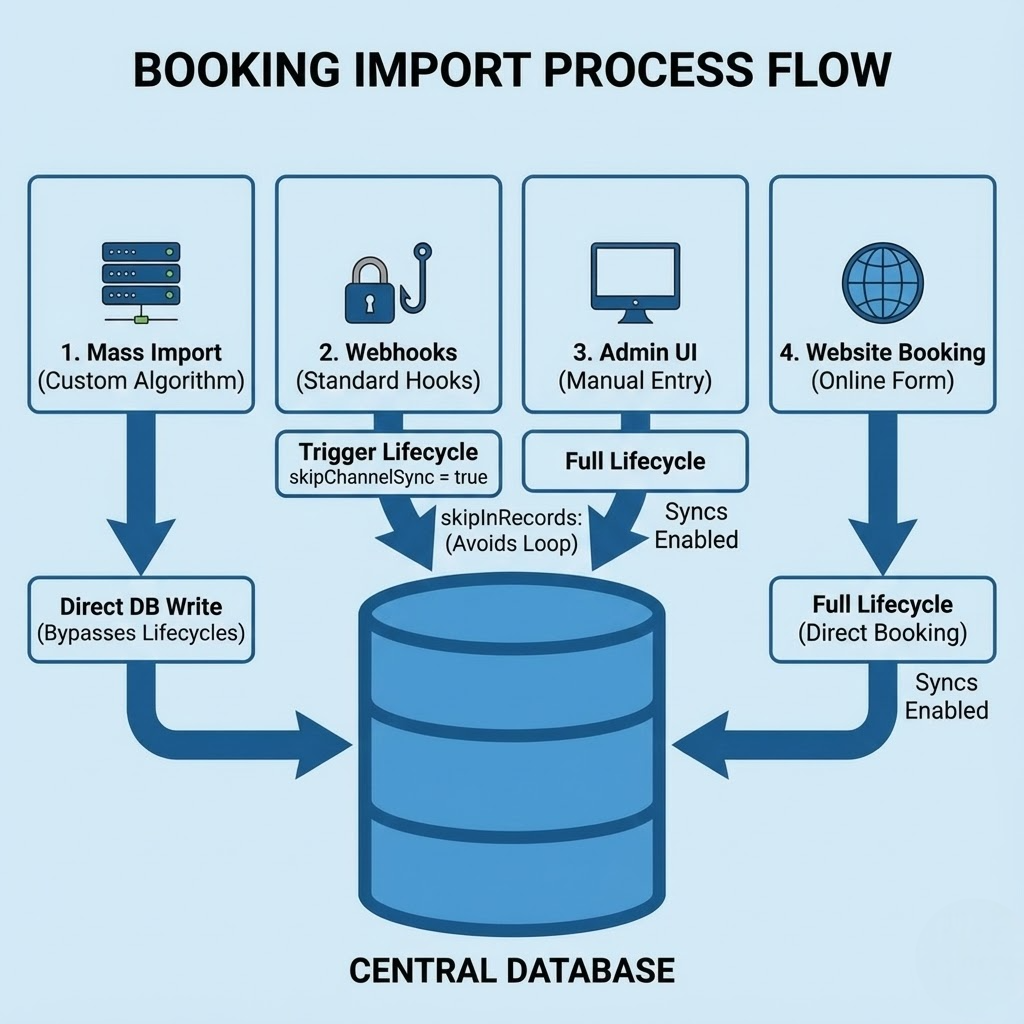
\includegraphics[width=\textwidth]{booking_import_flowchart.jpg}
    \caption{Μέθοδοι εισαγωγής κρατήσεων στην πλατφόρμα.}
    \label{fig:booking-import}
\end{figure}

\subsubsection{Α) Mass Import (Property Syncing)}

Κατά την αρχική εισαγωγή ή τον περιοδικό συγχρονισμό, η πλατφόρμα χρειάζεται να εισάγει εκατοντάδες ή χιλιάδες κρατήσεις. Χρησιμοποιείται η \code{payload.db.create()} και \code{payload.db.updateOne()} αντί των standard methods, παρακάμπτοντας τα hooks για βέλτιστη απόδοση.

\begin{lstlisting}[caption={Mass import με direct DB operations}]
const syncBookingsOperations = async (
  bookingsToCreate: RequiredDataFromCollectionSlug<"bookings">[],
  bookingsToUpdate: Array<{
    id: number;
    data: RequiredDataFromCollectionSlug<"bookings">;
  }>,
  bookingsToDelete: Booking[]
) => {
  // CREATE - Direct DB, bypassing lifecycle
  for (const booking of bookingsToCreate) {
    await payload.db.create({
      collection: "bookings",
      data: dtoPayloadToPayloadDb(booking),
    });
  }

  // UPDATE - Direct DB, bypassing lifecycle
  for (const { id, data } of bookingsToUpdate) {
    await payload.db.updateOne({
      collection: "bookings",
      id: id,
      data: dtoPayloadToPayloadDb(data),
    });
  }
};
\end{lstlisting}

\subsubsection{Β) Webhook Updates (Channel Manager Triggers)}

Όταν μια κράτηση δημιουργείται ή ενημερώνεται στο Beds24, η πλατφόρμα λαμβάνει ένα webhook notification. Κρίσιμο είναι το \code{skipChannelSync} flag:

\begin{lstlisting}[caption={Αποτροπή infinite loop με skipChannelSync flag}]
const createBookingRes = await payload.create({
  collection: "bookings",
  data: { ...dtoPayloadToPayloadDb(newBooking), skipChannelSync: true },
  req: { transactionID: transactionId },
});
\end{lstlisting}

\subsubsection{Γ) UI-Based Booking Creation}

Όταν ένας χρήστης δημιουργεί κράτηση μέσω του UI, εκτελείται το πλήρες lifecycle συμπεριλαμβανομένου του υπολογισμού προμηθειών:

\begin{figure}[H]
    \centering
    \includegraphics[width=0.8\textwidth]{commission_structure.png}
    \caption{Τριπλή δομή προμηθειών (Three-Tier Commission Structure).}
    \label{fig:commission-structure}
\end{figure}

\begin{lstlisting}[caption={Υπολογισμός commission}]
export const computeCommissionOfPlan = (
  booking: Partial<Booking>,
  plan: Plan
): number => {
  const bookingTotal = booking.pricing?.totalAmount ?? 0;

  if (booking.excludedFromCommission) return 0;

  if (plan.planCommission?.commissionType === "percentage") {
    const percentage = plan.planCommission.commissionPercentage ?? 0;
    return Math.round(bookingTotal * (percentage / 100) * 100) / 100;
  } else {
    return plan.planCommission?.fixedCommission ?? 0;
  }
};
\end{lstlisting}

\subsubsection{Δ) Website Booking Creation}

Για κρατήσεις από το generated website, το πεδίο \code{source} ορίζεται αντίστοιχα (\code{websitePlatform}, \code{websiteManager}, \code{websiteOwner}).

\begin{figure}[H]
    \centering
    \includegraphics[width=\textwidth]{booking_sync.png}
    \caption{Ροή δεδομένων συγχρονισμού κρατήσεων με το Beds24.}
    \label{fig:booking-sync}
\end{figure}

\section{Μηχανισμός Auto Actions}
\label{sec:auto-actions}

Το σύστημα Auto Actions είναι η «καρδιά» του αυτοματισμού της πλατφόρμας.

\subsection{Κατηγορίες Auto Actions}
\label{subsec:auto-action-categories}

Υπάρχουν τρεις διακριτοί τύποι:

\begin{enumerate}
    \item \textbf{Notifications to Users:} Ειδοποιήσεις προς τους χρήστες της πλατφόρμας (Managers, Owners, Staff).
    \item \textbf{Property Notifications to Guests:} Μηνύματα προς τους επισκέπτες (π.χ. οδηγίες άφιξης).
    \item \textbf{Simple Template:} Πρότυπα κειμένου χωρίς trigger condition, για χειροκίνητη αποστολή μέσω Chat.
\end{enumerate}

\subsection{Κανάλια Επικοινωνίας}
\label{subsec:communication-channels}

\begin{itemize}
    \item \textbf{Για Guests:} OTA Message (μέσω API καναλιού) ή Email.
    \item \textbf{Για Users:} Telegram. Η αρχιτεκτονική επιτρέπει εύκολη προσθήκη νέων καναλιών (WhatsApp, SMS).
\end{itemize}

\begin{figure}[H]
    \centering
    \includegraphics[width=\textwidth]{auto_actions.png}
    \caption{Διάγραμμα ροής εκτέλεσης των Auto Actions.}
    \label{fig:auto-actions}
\end{figure}

\subsection{Μηχανισμός Προτύπων (Template Engine)}
\label{subsec:template-engine}

Αναπτύχθηκε custom Template Engine με τις εξής δυνατότητες:

\begin{description}
    \item[Variable Replacement:] Σύνταξη \code{[object.property]} για πρόσβαση σε εμφωλευμένα δεδομένα
    \item[Conditional Logic:] Σύνταξη \code{\{condition?? result\}} για εμφάνιση κειμένου υπό συνθήκη
    \item[Date Formatting:] Αυτόματη αναγνώριση και μορφοποίηση ημερομηνιών
\end{description}

\begin{lstlisting}[style=text,caption={Παράδειγμα Template για νέα κράτηση}]
Νέα κράτηση:
🏠 Επιβεβαιωμένη κράτηση - [property.title]

👤 [booking.bookingHolder.firstName] [booking.bookingHolder.lastName]
👪 [booking.resource.adults] Ενήλικες, [booking.resource.children] Παιδιά
📆 Από [booking.resource.checkIn] έως [booking.resource.checkOut]

{user.settings.features.bookings.prices!=="none"?? 
  💰 Τιμή: €[booking.pricing.totalAmount]}

{user.settings.features.messages.visibility!=="none"?? 
  🗨 Μηνύματα: [link-booking-chat]}
\end{lstlisting}

\subsection{Time-based Triggers (Cron Jobs)}
\label{subsec:time-based-triggers}

\begin{table}[H]
\centering
\caption{Υποστηριζόμενοι Time-based Trigger Types}
\label{tab:trigger-types}
\begin{tabular}{@{}lll@{}}
\toprule
\textbf{Trigger Type} & \textbf{Περιγραφή} & \textbf{Πεδίο Κράτησης} \\
\midrule
\code{before-checkin} & Πριν την άφιξη & \code{resource.checkInStartOfDay} \\
\code{after-checkout} & Μετά την αναχώρηση & \code{resource.checkOutStartOfDay} \\
\code{after-cancellation} & Μετά την ακύρωση & \code{cancellationDate} \\
\code{after-new-booking} & Μετά τη νέα κράτηση & \code{reservationDate} \\
\bottomrule
\end{tabular}
\end{table}

\begin{lstlisting}[caption={Αλγόριθμος υπολογισμού χρονικού παραθύρου}]
const now: Date = new Date();
let fromDate: Date;
let toDate: Date;

if (triggerType.includes("before")) {
  // before: [now + interval, now + interval + window]
  fromDate = addHours(now, autoAction.timeInterval);
  toDate = addHours(now, autoAction.timeInterval + autoAction.timeWindow);
} else if (triggerType.includes("after")) {
  // after: [now - interval - window, now - interval]
  fromDate = subHours(now, autoAction.timeInterval + autoAction.timeWindow);
  toDate = subHours(now, autoAction.timeInterval);
}
\end{lstlisting}

\begin{figure}[H]
    \centering
    \includegraphics[width=\textwidth]{time_based_triggers_scenario.png}
    \caption{Σενάρια λειτουργίας Time-based Triggers για κράτηση τελευταίας στιγμής.}
    \label{fig:time-triggers}
\end{figure}

\subsection{Αρχιτεκτονική Cron Jobs}
\label{subsec:cron-architecture}

\begin{table}[H]
\centering
\caption{Scheduled Cron Jobs της πλατφόρμας}
\label{tab:cron-jobs}
\begin{tabular}{@{}llll@{}}
\toprule
\textbf{Cron Job} & \textbf{Συχνότητα} & \textbf{Αρχείο} & \textbf{Σκοπός} \\
\midrule
\code{everyHourCron} & Κάθε ώρα & \code{everyHourCron.ts} & Time-based Auto Actions \\
\code{everyNightCron} & Κάθε βράδυ & \code{everyNightCron.ts} & Token refresh, Full sync \\
\code{everyMonthCron} & Αρχή μήνα & \code{everyMonthCron.ts} & Billing records \\
\bottomrule
\end{tabular}
\end{table}

\section{Σύστημα Χρέωσης και Τιμολόγησης}
\label{sec:billing-system}

\subsection{Αρχιτεκτονική Χρέωσης}
\label{subsec:billing-architecture}

Το σύστημα billing δημιουργεί χρεώσεις ανά χρήστη στο τέλος κάθε μήνα:

\begin{itemize}
    \item \textbf{Owner Bill:} Ο Owner (Debtor) οφείλει στον Manager (Creditor)
    \item \textbf{Manager Bill:} Ο Manager (Debtor) οφείλει στην Πλατφόρμα (Creditor)
\end{itemize}

\subsection{Ανάλυση Χρεώσεων}
\label{subsec:pricing-breakdown}

\begin{table}[H]
\centering
\caption{Τύποι χρεώσεων Billing}
\label{tab:billing-types}
\begin{tabular}{@{}lll@{}}
\toprule
\textbf{Τύπος} & \textbf{Περιγραφή} & \textbf{Υπολογισμός} \\
\midrule
\code{propertyCommission} & Ανά ακίνητο & count $\times$ pricePerProperty \\
\code{unitCommission} & Ανά δωμάτιο & count $\times$ pricePerUnit \\
\code{bookingsCommission} & Προμήθεια κρατήσεων & $\sum$ commissions \\
\bottomrule
\end{tabular}
\end{table}

\subsection{Σύστημα Ελέγχου Πρόσβασης}
\label{subsec:access-control}

Η πλατφόρμα υλοποιεί έλεγχο πρόσβασης σε δύο άξονες:
\begin{enumerate}
    \item \textbf{Ρόλος Χρήστη:} platform-user, manager, owner, staff
    \item \textbf{Χαρακτηριστικά Πλάνου:} Ρυθμίσεις από τον Manager για κάθε Owner/Staff
\end{enumerate}

\begin{figure}[H]
    \centering
    \includegraphics[width=0.9\textwidth]{access_control_decision_tree.png}
    \caption{Decision tree για τον έλεγχο πρόσβασης.}
    \label{fig:access-control}
\end{figure}

\section{Αυτοματοποιημένη Παραγωγή Ιστοσελίδων}
\label{sec:website-generation}

\subsection{Δομή και Λειτουργία Website}
\label{subsec:website-structure}

Το παραγόμενο website ακολουθεί βελτιστοποιημένη δομή τριών σελίδων:

\begin{enumerate}
    \item \textbf{Home Page (/):} Multi-room search, property cards, filtering
    \item \textbf{Property Page (/properties/[id]):} Gallery, description, AI Chat Bubble
    \item \textbf{Booking Page (/booking/[id]):} Λεπτομέρειες κράτησης, self-service
\end{enumerate}

\subsection{Website API Endpoints}
\label{subsec:website-api}

\begin{table}[H]
\centering
\caption{Website API Endpoints}
\label{tab:website-api}
\begin{tabular}{@{}lll@{}}
\toprule
\textbf{Endpoint} & \textbf{Method} & \textbf{Σκοπός} \\
\midrule
\code{/api/website/properties} & GET & Λίστα καταλυμάτων \\
\code{/api/website/properties/[id]} & GET & Λεπτομέρειες \\
\code{/api/website/availability} & POST & Έλεγχος διαθεσιμότητας \\
\code{/api/website/booking} & POST & Δημιουργία κράτησης \\
\code{/api/website/booking/[id]} & GET & Λεπτομέρειες κράτησης \\
\bottomrule
\end{tabular}
\end{table}

\section{Περιβάλλον Χρήστη (Platform UI)}
\label{sec:platform-ui}

\subsection{Dashboard και Calendar}
\label{subsec:calendar}

Το ημερολόγιο σχεδιάστηκε ως «Easy Calendar» με:

\begin{itemize}
    \item \textbf{Drag and Drop:} Μετακίνηση κρατήσεων με τη βιβλιοθήκη \code{@dnd-kit}~\cite{dndkit}
    \item \textbf{Infinite Scrolling:} Οριζόντια (ημερομηνίες) και κάθετα (properties)
    \item \textbf{Επιλογή Εύρους:} Μαζική αλλαγή τιμών και διαθεσιμότητας
    \item \textbf{Φίλτρα Properties:} Επιλογή συγκεκριμένων καταλυμάτων
\end{itemize}

\subsection{Σύστημα Μηνυμάτων}
\label{subsec:messages}

Το Chat υποστηρίζει:
\begin{itemize}
    \item Άμεση επικοινωνία με φιλοξενούμενους μέσω OTAs
    \item Χρήση Simple Templates με auto-fill
    \item Βελτίωση κειμένου μέσω AI («Improve with AI»)
    \item Infinite scrolling και αναζήτηση
\end{itemize}

% ============================================================================
% CHAPTER 5: RESULTS
% ============================================================================
\chapter{Αποτελέσματα}
\label{chap:results}

\section{Παρουσίαση της Πλατφόρμας}
\label{sec:platform-presentation}

Η πλατφόρμα προσφέρει ένα μοντέρνο, responsive περιβάλλον εργασίας. Τα παρακάτω screenshots παρουσιάζουν την οπτική γωνία ενός χρήστη με πλήρη δικαιώματα (Admin/Manager).

\begin{figure}[H]
    \centering
    \fbox{\parbox{0.9\textwidth}{\centering\vspace{3cm}\textit{[Screenshot: Calendar Page]}\vspace{3cm}}}
    \caption{Η σελίδα του Ημερολογίου (Calendar).}
    \label{fig:calendar-page}
\end{figure}

\begin{figure}[H]
    \centering
    \fbox{\parbox{0.9\textwidth}{\centering\vspace{3cm}\textit{[Screenshot: Messages Page]}\vspace{3cm}}}
    \caption{Η σελίδα των Μηνυμάτων με AI capabilities.}
    \label{fig:messages-page}
\end{figure}

\section{Παρουσίαση του Generated Website}
\label{sec:website-presentation}

\begin{figure}[H]
    \centering
    \fbox{\parbox{0.9\textwidth}{\centering\vspace{3cm}\textit{[Screenshot: Website Generation Admin Panel]}\vspace{3cm}}}
    \caption{Διαδικασία παραγωγής Website από το περιβάλλον του διαχειριστή.}
    \label{fig:website-generation}
\end{figure}

\begin{figure}[H]
    \centering
    \fbox{\parbox{0.9\textwidth}{\centering\vspace{3cm}\textit{[Screenshot: Guest Website Navigation]}\vspace{3cm}}}
    \caption{Πλοήγηση επισκέπτη στην παραγόμενη ιστοσελίδα.}
    \label{fig:website-navigation}
\end{figure}

\begin{figure}[H]
    \centering
    \fbox{\parbox{0.9\textwidth}{\centering\vspace{3cm}\textit{[Screenshot: AI \& LLM Capabilities]}\vspace{3cm}}}
    \caption{Δυνατότητες AI και LLM για την εξυπηρέτηση επισκεπτών.}
    \label{fig:website-ai}
\end{figure}

\section{Τεχνικές Προκλήσεις και Λύσεις}
\label{sec:technical-challenges}

\subsection{Συγχρονισμός Δεδομένων με External APIs}
\label{subsec:sync-challenge}

\textbf{Πρόβλημα:} Διατήρηση συνέπειας μεταξύ τοπικής βάσης και Beds24.

\textbf{Λύση:} Υιοθέτηση στρατηγικής όπου το Beds24 είναι η κύρια πηγή αλήθειας για δεδομένα κρατήσεων, με merge logic για internal fields.

\subsection{Αποφυγή Infinite Loops}
\label{subsec:loop-prevention}

\textbf{Πρόβλημα:} Two-way sync δημιουργεί κύκλους.

\textbf{Λύση:} Χρήση \code{skipChannelSync} flag για αποτροπή reverse-update.

\subsection{Απόδοση Μαζικών Εισαγωγών}
\label{subsec:mass-import-performance}

\textbf{Πρόβλημα:} Εισαγωγή ~60.000 records με standard lifecycle απαιτεί ώρες.

\textbf{Λύση:} Hybrid strategy με direct DB operations για bulk, standard lifecycle για μεμονωμένες αλλαγές.

\begin{table}[H]
\centering
\caption{Σύγκριση στρατηγικών εισαγωγής}
\label{tab:import-comparison}
\begin{tabular}{@{}lll@{}}
\toprule
\textbf{Περίπτωση} & \textbf{Μέθοδος} & \textbf{Πλεονέκτημα} \\
\midrule
Mass Property Import & Direct DB & 50$\times$ ταχύτερο \\
Mass Rate Import & Bulk Insert & 1 query για χιλιάδες records \\
Individual Updates & Standard Lifecycle & Consistency, hooks \\
\bottomrule
\end{tabular}
\end{table}

% ============================================================================
% CHAPTER 6: DISCUSSION
% ============================================================================
\chapter{Συζήτηση}
\label{chap:discussion}

\section{Αξιολόγηση Τεχνολογικών Επιλογών}
\label{sec:tech-evaluation}

Η υιοθέτηση του μοντέλου «Backend Framework» με το PayloadCMS v3 και η χρήση Serverless υποδομών απέδειξε ότι είναι δυνατή η ανάπτυξη πολύπλοκων εφαρμογών με ελάχιστους πόρους.

\begin{table}[H]
\centering
\caption{Αξιολόγηση τεχνολογικών επιλογών}
\label{tab:tech-evaluation}
\begin{tabular}{@{}L{3cm}L{5cm}L{5cm}@{}}
\toprule
\textbf{Επιλογή} & \textbf{Όφελος} & \textbf{Trade-off} \\
\midrule
PayloadCMS v3 & Rapid development, type-safety & Lock-in σε ecosystem \\
PostgreSQL & ACID transactions, complex queries & Setup complexity \\
Serverless & Zero DevOps, auto-scaling & Cold starts \\
Next.js App Router & SSR, Server Actions & Learning curve \\
\bottomrule
\end{tabular}
\end{table}

\section{Μελλοντικές Βελτιώσεις}
\label{sec:future-work}

\subsection{Βελτίωση UX στο Admin Panel}
\begin{itemize}
    \item GUI Builder για Templates με drag-and-drop
    \item Visual Auto Action Editor με flow-chart style
    \item Wizard-style user creation
\end{itemize}

\subsection{Επέκταση Channel Manager Support}
\begin{itemize}
    \item Hostaway (υψηλή προτεραιότητα)
    \item Lodgify (μεσαία προτεραιότητα)
    \item Custom/Direct integrations
\end{itemize}

\subsection{Mobile Application}
\begin{itemize}
    \item Push notifications για νέες κρατήσεις
    \item Quick actions (approve, respond)
    \item Offline calendar viewing
\end{itemize}

\subsection{Advanced Analytics Dashboard}
\begin{itemize}
    \item Revenue per property/room
    \item Occupancy rates over time
    \item Booking source distribution
\end{itemize}

% ============================================================================
% CHAPTER 7: CONCLUSIONS
% ============================================================================
\chapter{Συμπεράσματα}
\label{chap:conclusions}

\section{Επίτευξη Στόχων}
\label{sec:goal-achievement}

Η πλατφόρμα Lunarety V2 επιτυγχάνει τον στόχο της να γεφυρώσει το χάσμα μεταξύ Channel Managers και ιδιοκτητών ακινήτων.

\begin{table}[H]
\centering
\caption{Κύρια επιτεύγματα της πλατφόρμας}
\label{tab:achievements}
\begin{tabular}{@{}L{3.5cm}L{4.5cm}L{4.5cm}@{}}
\toprule
\textbf{Στόχος} & \textbf{Υλοποίηση} & \textbf{Αποτέλεσμα} \\
\midrule
Two-way sync & Webhooks + API integration & Real-time consistency \\
Αυτοματοποίηση & Auto Actions (time/instant) & 80\% μείωση εργασιών \\
Ιεραρχία χρηστών & 4-level system & Ανεξαρτησία διαχείρισης \\
Generated websites & One-click Vercel deploy & 2-min deployment \\
AI integration & OpenRouter + Vercel AI SDK & 24/7 ψηφιακή εξυπηρέτηση \\
\bottomrule
\end{tabular}
\end{table}

\section{Τεχνικά Συμπεράσματα}
\label{sec:technical-conclusions}

\textbf{Αρχιτεκτονικές αποφάσεις που δικαιώθηκαν:}

\begin{enumerate}
    \item \textbf{PayloadCMS v3:} Το hook system αποδείχθηκε ιδανικό για complex business logic.
    \item \textbf{PostgreSQL vs MongoDB:} Οι complex queries για billing και access control θα ήταν δυσκολότερες με document-based storage.
    \item \textbf{Serverless Architecture:} Απλοποίησε το deployment και μείωσε τα operation costs.
    \item \textbf{Monorepo Structure:} Διευκόλυνε τη συντήρηση και την κοινή χρήση τύπων.
\end{enumerate}

\section{Βασικά Διδάγματα}
\label{sec:lessons-learned}

\begin{enumerate}
    \item \textbf{Direct DB Operations για Mass Import:} Η παράκαμψη του lifecycle για bulk operations είναι απαραίτητη.
    \item \textbf{Flag-based Loop Prevention:} Απλή και αποτελεσματική λύση για two-way sync.
    \item \textbf{Feature-based Access Control:} Επιτρέπει παραμετροποίηση ανά Manager.
    \item \textbf{AI as Enhancement:} Βελτιώνει την εμπειρία χωρίς να αντικαθιστά ανθρώπινη κρίση.
\end{enumerate}

% ============================================================================
% BIBLIOGRAPHY
% ============================================================================
\printbibliography[heading=bibintoc,title={Βιβλιογραφία}]

% ============================================================================
% APPENDICES
% ============================================================================
\appendix

\chapter{Δομή Webhook Payload}
\label{app:webhook}

\begin{lstlisting}[caption={Παράδειγμα Webhook Payload από Beds24}]
{
  "booking": {
    "id": 12345,
    "arrival": "2025-01-01",
    "departure": "2025-01-05",
    "status": "confirmed"
  },
  "messages": [...]
}
\end{lstlisting}

\chapter{Παράδειγμα Auto Action Query}
\label{app:auto-action-query}

\begin{lstlisting}[caption={Αναζήτηση κρατήσεων για before-checkin trigger}]
const whereClause = {
  'resource.checkInStartOfDay': {
    greater_than_equal: fromDate.toISOString(),
    less_than_equal: toDate.toISOString(),
  },
  'logging.automationTracking.triggeredAutomations': {
    not_in: [autoAction.id],
  }
}
\end{lstlisting}

\end{document}

